\subsection{Triangles In A Cube}

My dad gave me this problem as a simple problem with a fast answer and said it could be solved within 10 seconds, although I found a way of solving this even faster. I would have expected almost anyone to be able to solve this, although I have been surprised that normal people have pretty poor geometric reasoning abilities. I rate this problem a 1/10 in difficulty.

How many equilateral triangles can be formed by connecting three vertices of a cube?

\textbf{Hints:}

\begin{enumerate}
	\item Connecting any three distinct vertices on the same face will form a right-angled triangle.
	\item Equilateral triangles have rotational symmetry of order 3 - where on a cube do you find such a symmetry?
\end{enumerate}

\textbf{Solution:}

Place three points overlapping at a vertex of the cube. There are three edges connected to this vertex, and we move the points along each of the edges. If all points move along their edge at the same speed then they will form an equilateral triangle by symmetry. Eventually they hit the vertex at the end of the edge, and thus we have found three vertices that form an equilateral triangle. This gives one triangle per vertex, therefore the final answer is 8. We have not shown that these are the only such triangles, although it is not hard to convince yourself by visualising it. The next method proves that these are all the equilateral triangles however.

There are 24 orientation-preserving symmetries of the vertices of a cube, and these form the $O$ group. The vertices of an equilateral triangle have 3 orientation-preserving symmetries and form the $C_3$ group. The quotient set $O/C_3$ has size $\left| \frac{O}{C_3} \right| = \frac{|O|}{|C_3|} = \frac{24}{3} = 8$, and this is the number of triples of vertices with threefold rotational symmetry, in other words, the equilateral triangles.

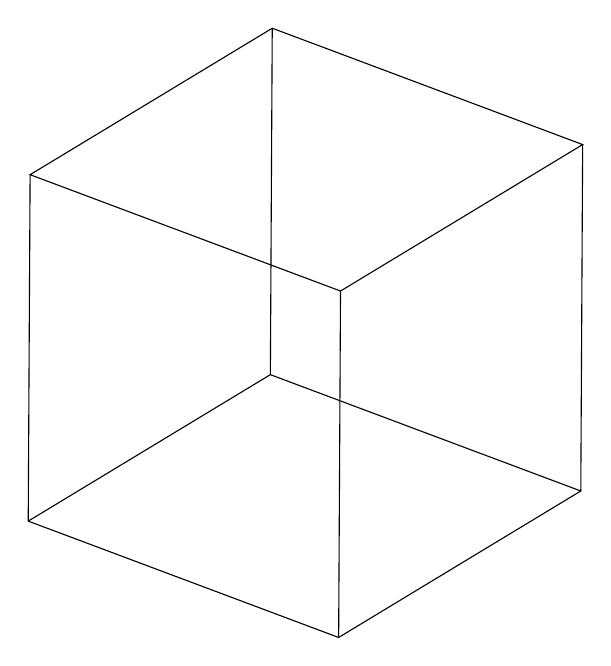
\begin{tikzpicture}[scale=5]
	% Angles used:
	% a = -0.6
	% b = -0.3
	% c =  0.4
	
	% Basis vectors used;
	% 0.47509207, -0.00476773, -0.87992318
	%-0.53942356,  0.78847323, -0.29552021
	% 0.69520483,  0.6150506 ,  0.37202555
	
	\coordinate (V1) at ( 0.00000000,  0.00000000);
	\coordinate (V2) at ( 0.61505060,  0.37202555);
	\coordinate (V3) at ( 0.78847323, -0.29552021);
	\coordinate (V4) at ( 1.40352383,  0.07650535);
	\coordinate (V5) at (-0.00476773, -0.87992318);
	\coordinate (V6) at ( 0.61028287, -0.50789762);
	\coordinate (V7) at ( 0.78370550, -1.17544338);
	\coordinate (V8) at ( 1.39875610, -0.80341783);
	
	\draw (V2) -- (V4) -- (V3) -- (V1) -- (V2);
	\draw (V5) -- (V7) -- (V8) -- (V6) -- (V5);
	\draw (V1) -- (V5);
	\draw (V2) -- (V6);
	\draw (V3) -- (V7);
	\draw (V4) -- (V8);
	
	
\end{tikzpicture}

\textbf{Extensions and Comments:}